\chapter [Sprawozdzanie 2]{Opis i implementacja algorytmów} 
\fancyhead[C]{OPIS I IMPLEMENTACJA ALHGORYTMÓW}
\fancyhead[L]{}
\fancyhead[R]{}
\textbf{Problem (zdefiniowany na podstawie \cite{prim2}):}\\
Znalezienie takiego podzbioru krawędzi spójnego grafu nieskierowanego ważonego, który zapewnia połączenie każdego wierzchołka grafu z dowolnym innym i ponadto posiada najmniejszą możliwą sumę wag krawędzi. \\Taki podzbiór nie może zawierać żadnego cyklu, a zatem jest drzewem i musi zawierać dokładnie \emph{n-1} krawędzi dla grafu o \emph{n} wierzchołkach. Drzewo takie ze względu na minimalną sumę wag nazywane jest minimalnym drzewem rozpinającym.

\section{Algorytm Prima}
\textbf{Dane wejściowe:} \\ 
Spójny ważony graf nieskierowany, zawierający n wierzchołków, gdzie $n \geqslant 2$.\\
Graf jest reprezentowany przez macierz sąsiedztwa \emph{graph}, gdzie element \emph{graph[i][j]} reprezentuje wagę krawędzi łączącej wierzchołki \emph{i} oraz \emph{j}.\\

\subsection{Pseudokod zaimplementowanego algorytmu}
\begin{enumerate}
	\item Inicjalizacja
	\begin{itemize}
		\item Utwórz pusty zbiór zawierający krawędzie minimalnego drzewa rozpinającego: \\ \emph{minSpanningTree}.
		\item Zainicjalizuj pustą listę odwiedzonych wierzchołków: \emph{visitedVertices}.
		\item Utwórz pustą listę krawędzi incydentnych do odwiedzonych wierzchołków: \emph{adjacencyEdges}.
	\end{itemize}

	\item Losuj wierzchołek początkowy: \emph{startV}.
	\item Oznacz wierzchołek początkowy jako odwiedzony poprzez dodanie go do listy wierzchołków odwiedzonych \emph{visitedVertices}.
	\item Pobierz do zmiennej \emph{adjacencyEdges} posortowaną względem wag listę wszystkich krawędzi incydentnych do wierzchołka \emph{startV}.
	\item Dopóki lista \emph{visitedVertices} nie zawiera wszystkich wierzchołków grafu:
	\item[a.] Zainicjalizuj zmienną aktualnie rozpatrywanej krawędzi -- \emph{minEdge} -- poprzez pobranie najmniejszego elementu listy \emph{adjacencyEdges}.
	\item[b.1.] Jeśli lista odwiedzonych wierzchołków \emph{visitedVertices} nie zawiera jeszcze wierzchołka końcowego aktualnie rozpatrywanej krawędzi \emph{minEdge}:\\
	-- dodaj krawędź \emph{minEdge} do zbioru krawędzi minimalnego drzewa rozpinającego \emph{minSpanningTree}\\
	-- przypisz zmiennej \emph{startV} wartość wierzchołka końcowego krawędzi \emph{minEdge}\\
	-- oznacz wierzchołek końcowy krawędzi \emph{minEdge } jako odwiedzony \\
	-- usuń krawędź uwzględnioną w \emph{minSpanningTree} -- \emph{minEdge} -- z listy krawędzi incydentnych do odwiedzonych wierzchołków
	-- ustal aktualną listę nietworzących cyklu krawędzi incydentnych do wierzchołków odwiedzonych
	\item[b.2.] Jeśli lista odwiedzonych wierzchołków \emph{visitedVertices} zawiera już wierzchołek końcowy aktualnie rozpatrywanej krawędzi \emph{minEdge}:\\
	-- usuń krawędź tworzącą cykl z listy krawędzi incydentnych do odwiedzonych wierzchołków\\
\end{enumerate} 

%%%%%%%%%%%%%%%%%%%%%%%%%%%%%%%%%
\newpage
\subsection{Zasada działania zaimplementowanego algorytmu na przykładzie}
Poniżej znajduje się legenda oznaczeń wykorzystanych w opisie działania algorytmu na przykładzie.

\begin{figure}[htb!]
	\centering
	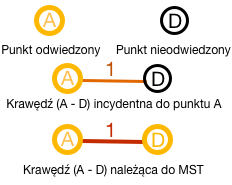
\includegraphics[width=0.4\textwidth]{tex/fig/legenda}
	\caption{Oznaczenia wykorzystane w opisie}
	\label{fig: legenda}
\end{figure}

Dany jest graf widoczny na rys.\ref{fig: g1}.  Wierzchołki oznaczono wielkimi literami alfabetu,\\ natomiast krawędziom nadano wagi $w\subseteq \{1,5\}$.\\

\begin{figure}[htb!]
	\centering
		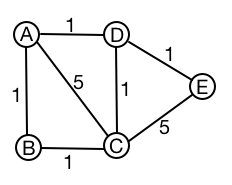
\includegraphics[width=0.4\textwidth]{tex/fig/graf1}
\caption{Graf wejściowy.}
\label{fig: g1}
\end{figure}

\textbf{Inicjalizacja}\\
Zbiór: \emph{minSpanningTree} =\{ \};\\
Lista wierzchołków odwiedzonych: \emph{visitedVertices} = [ ];\\
Lista krawędzi incydentnych: \emph{adjacencyEdges} = [ ];
\newpage
\textbf{Krok 1.}\\
Losowanie wierzchołka początkowego. W tym przypadku niech będzie to wierzchołek \textbf{A}.
\begin{center}
	\emph{startV} = A
\end{center}

\textbf{Krok 2.}\\
Oznaczenie wierzchołka \emph{startV} jako odwiedzony. 
\begin{figure}[htb!]
	\centering
	
\includegraphics[width=0.4\textwidth]{tex/fig/graf2}
	\caption{Prim -- Krok 2.}
	\label{fig: g2}
\end{figure}\\
Zbiór: \emph{minSpanningTree} =\{ \};\\
Lista wierzchołków odwiedzonych: \emph{visitedVertices} = [ A ];\\
Lista krawędzi incydentnych: \emph{adjacencyEdges} = [ ];\\

\textbf{Krok 3.}\\
Pobranie listy krawędzi incydentnych do wierzchołka \emph{startV}, które nie tworzą cyklu. 
\begin{figure}[htb!]
	\centering
	
\includegraphics[width=0.4\textwidth]{tex/fig/graf3}
	\caption{Prim -- Krok 3.}
	\label{fig: g3}
\end{figure}\\
Zbiór: \emph{minSpanningTree} =\{ \};\\
Lista wierzchołków odwiedzonych: \emph{visitedVertices} = [ A ];\\
Lista krawędzi incydentnych: \emph{adjacencyEdges} = [ (A -- D), (A -- B), (A -- C) ];\\

\textbf{Krok 4.}\\
Inicjalizacja \emph{minEdge} poprzez wybór pierwszego elementu posortowanej rosnąco listy krawędzi incydentnych \emph{adjacencyEdges}.\\
 \begin{center}
 	\emph{minEdge} = (A -- D)
 \end{center}

\textbf{Krok 5.}\\
Lista \emph{visitedVertices} nie zawiera jeszcze wierzchołka końcowego krawędzi \emph{minEdge} (D), dlatego:\\
-- Brak cyklu z krawędzią \emph{minEdge}\\
-- Dodanie krawędzi \emph{minEdge} do zbioru krawędzi minimalnego drzewa rozpinającego \emph{minSpanningTree}
 \begin{center}
Zbiór: \emph{minSpanningTree} =\{ (A -- D) \};
 \end{center}
-- przypisanie zmiennej \emph{startV} wartości wierzchołka końcowego krawędzi \emph{minEdge}
\begin{center}
	\emph{startV} = D
\end{center}
-- oznaczenie wierzchołka końcowego krawędzi \emph{minEdge } jako odwiedzony \\
-- usunięcie krawędzi uwzględnionej w \emph{minSpanningTree} -- \emph{minEdge} -- z listy krawędzi incydentnych do odwiedzonych wierzchołków \emph{adjacencyEdges}

\begin{center}
Lista wierzchołków odwiedzonych: \emph{visitedVertices} = [ A , D ];\\
Lista krawędzi incydentnych: \emph{adjacencyEdges} = [ (A -- B), (A -- C) ];\\
\end{center}
\begin{figure}[htb!]
	\centering
	
\includegraphics[width=0.4\textwidth]{tex/fig/graf4}
	\caption{Prim -- Krok 5.}
	\label{fig: g4}
\end{figure}
-- aktualizacja listy krawędzi incydentnych do odwiedzonych wierzchołków \emph{adjacencyEdges}
\begin{figure}[htb!]
	\centering
	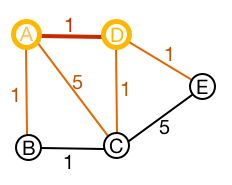
\includegraphics[width=0.4\textwidth]{tex/fig/graf5}
	\caption{Prim -- Krok 5 - aktualizacja listy krawędzi.}
	\label{fig: g5}
\end{figure}
\begin{center}
	Lista krawędzi incydentnych: \emph{adjacencyEdges} = [ (A -- B), (D -- C), (D -- E), (A -- C)];\\
\end{center}

\textbf{Krok 6.}\\
Aktualizacja \emph{minEdge} poprzez wybór pierwszego elementu posortowanej rosnąco listy krawędzi incydentnych \emph{adjacencyEdges}.\\
\begin{center}
	\emph{minEdge} = (A -- B)
\end{center}

\textbf{Krok 7.}\\
Lista \emph{visitedVertices} nie zawiera jeszcze wierzchołka końcowego krawędzi \emph{minEdge} (B), dlatego:\\
-- Brak cyklu z krawędzią \emph{minEdge}\\
-- Dodanie krawędzi \emph{minEdge} do zbioru krawędzi minimalnego drzewa rozpinającego \emph{minSpanningTree}
\begin{center}
	Zbiór: \emph{minSpanningTree} =\{ (A -- D), (A -- B) \};
\end{center}
-- przypisanie zmiennej \emph{startV} wartości wierzchołka końcowego krawędzi \emph{minEdge}
\begin{center}
	\emph{startV} = B
\end{center}
-- oznaczenie wierzchołka końcowego krawędzi \emph{minEdge } jako odwiedzony \\
-- usunięcie krawędzi uwzględnionej w \emph{minSpanningTree} -- \emph{minEdge} -- z listy krawędzi incydentnych do odwiedzonych wierzchołków \emph{adjacencyEdges}

\begin{center}
	Lista wierzchołków odwiedzonych: \emph{visitedVertices} = [ A , D , B];\\
	Lista krawędzi incydentnych: \emph{adjacencyEdges} = [ (D -- C), (D -- E), (A -- C) ];\\
\end{center}
\begin{figure}[htb!]
	\centering
	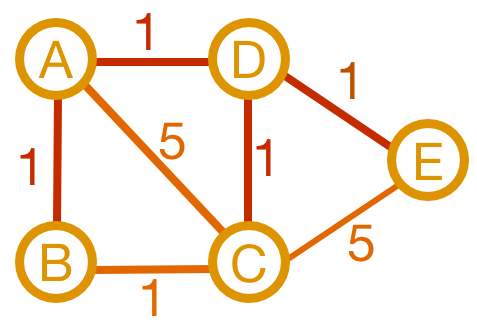
\includegraphics[width=0.4\textwidth]{tex/fig/graf6}
	\caption{Prim -- Krok 7.}
	\label{fig: g6}
\end{figure}
-- aktualizacja listy krawędzi incydentnych do odwiedzonych wierzchołków \emph{adjacencyEdges}
\begin{figure}[htb!]
	\centering
	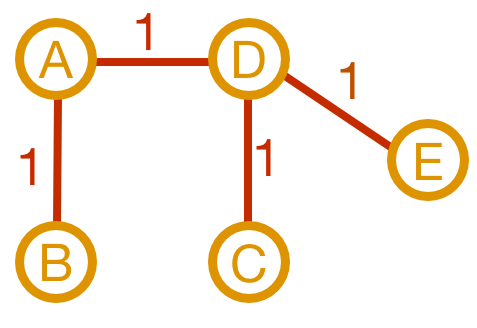
\includegraphics[width=0.4\textwidth]{tex/fig/graf7}
	\caption{Prim -- Krok 7 - aktualizacja listy krawędzi.}
	\label{fig: g7}
\end{figure}
\begin{center}
	Lista krawędzi incydentnych: \emph{adjacencyEdges} = [ (B -- C), (D -- C), (D -- E), (A -- C) ];\\
\end{center}

%%%%%%%%%%%%%%%%%%%%%%%%%%%%%%%%%%%%%%%%%%%%%%%%%%%%
\textbf{Krok 8.}\\
Aktualizacja \emph{minEdge} poprzez wybór pierwszego elementu posortowanej rosnąco listy krawędzi incydentnych \emph{adjacencyEdges}.\\
\begin{center}
	\emph{minEdge} = (B -- C)
\end{center}

\textbf{Krok 9.}\\
Lista \emph{visitedVertices} nie zawiera jeszcze wierzchołka końcowego krawędzi \emph{minEdge} (C), dlatego:\\
-- Brak cyklu z krawędzią \emph{minEdge}\\
-- Dodanie krawędzi \emph{minEdge} do zbioru krawędzi minimalnego drzewa rozpinającego \emph{minSpanningTree}
\begin{center}
	Zbiór: \emph{minSpanningTree} =\{ (A -- D), (A -- B), (B -- C) \};
\end{center}
-- przypisanie zmiennej \emph{startV} wartości wierzchołka końcowego krawędzi \emph{minEdge}
\begin{center}
	\emph{startV} = C
\end{center}
-- oznaczenie wierzchołka końcowego krawędzi \emph{minEdge } jako odwiedzony \\
-- usunięcie krawędzi uwzględnionej w \emph{minSpanningTree} -- \emph{minEdge} -- z listy krawędzi incydentnych do odwiedzonych wierzchołków \emph{adjacencyEdges}

\begin{center}
	Lista wierzchołków odwiedzonych: \emph{visitedVertices} = [ A , D , B, C];\\
	Lista krawędzi incydentnych: \emph{adjacencyEdges} = [ (D -- C), (D -- E), (A -- C) ];\\
\end{center}
\begin{figure}[htb!]
	\centering
	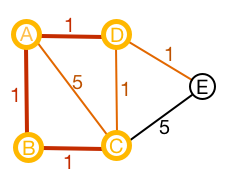
\includegraphics[width=0.4\textwidth]{tex/fig/graf8}
	\caption{Prim -- Krok 9.}
	\label{fig: g8}
\end{figure}
-- aktualizacja listy krawędzi incydentnych do odwiedzonych wierzchołków \emph{adjacencyEdges}
\begin{figure}[htb!]
	\centering
	
\includegraphics[width=0.4\textwidth]{tex/fig/graf9}
	\caption{Prim -- Krok 9 - aktualizacja listy krawędzi.}
	\label{fig: g9}
\end{figure}
\begin{center}
	Lista krawędzi incydentnych: \emph{adjacencyEdges} = [ (D -- C), (D -- E), (A -- C), (C -- E) ];\\
\end{center}
%%%%%%%%%%%%%%%%%%%%%%%%%%%%%%%%%%%%%%%%%%%%%%%%%%%%%%%%%%%%%%%%

\textbf{Krok 10.}\\
Aktualizacja \emph{minEdge} poprzez wybór pierwszego elementu posortowanej rosnąco listy krawędzi incydentnych \emph{adjacencyEdges}.\\
\begin{center}
	\emph{minEdge} = (D -- C)
\end{center}

\textbf{Krok 11.}\\
Lista \emph{visitedVertices} zawiera wierzchołek krawędzi \emph{minEdge} (C), dlatego:\\
-- Usunięcie krawędzi \emph{minEdge} z listy krawędzi incydentnych do odwiedzonych wierzchołków
\begin{center}
	Lista krawędzi incydentnych: \emph{adjacencyEdges} = [ (D -- E), (A -- C), (C -- E) ];
\end{center}

\begin{figure}[htb!]
	\centering
	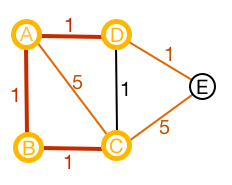
\includegraphics[width=0.4\textwidth]{tex/fig/graf10}
	\caption{Prim -- Krok 11.}
	\label{fig: g10}
\end{figure}
%%%%%%%%%%%%%%%%%%%%%%%%%%%%%%%%%%%%%%%%%%%%%%%%%%%%%%%%%%%%%%
\textbf{Krok 12.}\\
Aktualizacja \emph{minEdge} poprzez wybór pierwszego elementu posortowanej rosnąco listy krawędzi incydentnych \emph{adjacencyEdges}.\\
\begin{center}
	\emph{minEdge} = (D -- E)
\end{center}

\textbf{Krok 13.}\\
Lista \emph{visitedVertices} nie zawiera jeszcze wierzchołka końcowego krawędzi \emph{minEdge} (E), dlatego:\\
-- Brak cyklu z krawędzią \emph{minEdge}\\
-- Dodanie krawędzi \emph{minEdge} do zbioru krawędzi minimalnego drzewa rozpinającego \emph{minSpanningTree}
\begin{center}
	Zbiór: \emph{minSpanningTree} =\{ (A -- D), (A -- B), (B -- C), (D -- E) \};
\end{center}
-- przypisanie zmiennej \emph{startV} wartości wierzchołka końcowego krawędzi \emph{minEdge}
\begin{center}
	\emph{startV} = E
\end{center}
-- oznaczenie wierzchołka końcowego krawędzi \emph{minEdge } jako odwiedzony \\
-- usunięcie krawędzi uwzględnionej w \emph{minSpanningTree} -- \emph{minEdge} -- z listy krawędzi incydentnych do odwiedzonych wierzchołków \emph{adjacencyEdges}

\begin{center}
	Lista wierzchołków odwiedzonych: \emph{visitedVertices} = [ A , D , B, C, E];\\
	Lista krawędzi incydentnych: \emph{adjacencyEdges} = [ (C -- E), (A -- C) ];\\
\end{center}
-- aktualizacja listy krawędzi incydentnych do odwiedzonych wierzchołków \emph{adjacencyEdges}
\begin{figure}[htb!]
	\centering
	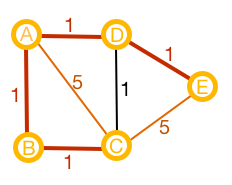
\includegraphics[width=0.4\textwidth]{tex/fig/graf11}
	\caption{Prim -- Krok 13.}
	\label{fig: g11}
\end{figure}
\begin{center}
	Lista krawędzi incydentnych: \emph{adjacencyEdges} = [ (C -- E), (A -- C) ];\\
\end{center}
\newpage
\textbf{Krok 14.}\\
Lista \emph{visitedVertices} zwiera wszystkie wierzchołki grafu wejściowego. W związku z tym otrzymano następujące drzewo rozpinające:\\
\begin{figure}[htb!]
	\centering
	
\includegraphics[width=0.4\textwidth]{tex/fig/graf12}
	\caption{Prim -- Krok 14 -- otrzymane MST.}
	\label{fig: g14}
\end{figure}
\newpage
\section{Składowe implementacji algorytmu}

\begin{table}[!hbp]
	\hspace{-60pt}
	\begin{tabular}{|C{5cm}|C{3cm}|C{9cm}|} \hline
		\textbf{Składowa}& \textbf{Rodzaj}& \textbf{Opis}\\ \hline
		rand & Zmienna pomocnicza  & Element odpowiedzialny za losowy wybór wierzchołka początkowego\\ \hline
		startV & Zmienna typu int  & Wierzchołek początkowy minimalnej krawędzi z listy \emph{adjacencyEdgesList}. Na początku przyjmuje wartość losową. \\ \hline
		visitedVertices & Lista elementów typu Integer  & Lista odwiedzonych wierzchołków grafu\\ \hline
		adjacencyEdgesList & Lista elementów typu Edge& Lista krawędzi incydentnych do odwiedzonych wierzchołków grafu\\
		&ArrayList<Edge>&\\ \hline
		minSpanningTree & Zbiór Set<Edge>  & Zbiór krawędzi, tworzących minimalne drzewo rozpinające\\ \hline
		minEdge & Zmienna typu Edge  & Obiekt klasy \emph{ Edge} (krawędź), zawierający minimalną krawędź  z listy \emph{adjacencyEdgesList} \\ \hline
		setVertexVisited(int vertex, ArrayList<Integer> list) & metoda & Metoda dodająca wierzchołek \emph{vertex} do listy wierzchołków odwiedzonych \emph{list} jeśli lista ta nie zawiera wierzchołka \emph{vertex}\\ \hline
		getAllAdjacencyEdges(int vertex, int[][] graph) & Metoda zwracająca listę obiektów Edge  & Metoda odpowiedzialna za ustalenie listy krawędzi incydentnych do odwiedzonych punktów \emph{adjacencyEdgesList}. Dla każdego wierzchołka \emph{i} $\subseteq V$ grafu weryfikuje czy dany wierzchołek \emph{i} tworzy krawędź z wierzchołkiem \emph{vertex}. Jeśli krawędź taka istnieje i lista \emph{visitedVertices} nie zawiera wierzchołka \emph{i}, to do listy \emph{adjacencyEdgesList} zostaje dodana krawędź (\emph{vertex} -- \emph{i})\\ \hline
		minSpanningTree.add(minEdge) & Operacja na zbiorze minSpanningTree & Operacja polegająca na dodaniu do zbioru \emph{minSpanningTree} minimalnej krawędzi \emph{minEdge}\\ \hline
	\end{tabular}
	\caption{Składowe implementacji algorytmu Prima}
	\label{skladowe}
\end{table}
\newpage
\begin{table}[!hbp]
	\hspace{-60pt}
	\begin{tabular}{|C{5cm}|C{3cm}|C{9cm}|} \hline
		\textbf{Składowa}& \textbf{Rodzaj}& \textbf{Opis}\\ \hline
		adjacencyEdges.remove(minEdge) & Operacja na liście \emph{adjacencyEdges} & Operacja polegająca na usunięciu z listy krawędzi \emph{adjacencyEdges} krawędzi \emph{minEdge}\\ \hline
		Edge & Klasa &Jest to klasa, której obiekty reprezentują krawędzie grafu. Ich atrybutami są: wierzchołek początkowy i końcowy krawędzi oraz jej waga. Klasa implementuje również metodę odpowiedzialną za sortowanie obiektów Edge znajdujących się w liście (metoda compareTo(Edge arg)) oraz metodę odpowiedzialną za wypisanie danej krawędzi (metoda toString()).\\ \hline
		
	\end{tabular}
	\caption{Składowe implementacji algorytmu Prima c.d.}
	\label{skladowe2}
\end{table}


\begin{center}
\textbf{Uwagi}
\end{center}
\begin{itemize}
\item W celu realizacji projektu zaistniała również konieczność implementacji modułu generującego macierz sąsiedztwa reprezentującą graf oraz zapisującego ją do pliku tekstowego na pulpicie. 
Ponadto należało zaimplementować mechanizm odpowiedzialny za odczyt wygenerowanej macierzy z pliku.
\item W procesie implementacji algorytmu Prima bazowano na następujących źródłach: \cite{prim} oraz \cite{prim3}. Źródła te miały wpływ na wybór odpowiednich struktur danych oraz na samo zrozumienie istoty algorytmu.
\end{itemize}


\newpage